\chapter{Results and Discussion}\label{results-and-discussion}

\section{Scalability Improvements}\label{results-and-discussion:s:scalability-improvements}

\subsection{Cost Rundown}\label{results-and-discussion:ss:cost-rundown}

The Infrastructure used to provide the Application to the Client is not free. As such, before comparing the older and newer architectures, the costs associated with each individual item are presented in \Cref{tab:individual-cost-aws-old} and \Cref{tab:individual-cost-aws-new}, respectively. 


\begin{table}[!htbp]
  
  \label{tab:individual-cost-aws-old}
  \resizebox{\textwidth}{!}{%
  \begin{tabular}{llccc}
  \hline
  \rowcolor[HTML]{EFEFEF} 
  Name               & Description                                                                   & \multicolumn{1}{l}{\cellcolor[HTML]{EFEFEF}\begin{tabular}[c]{@{}l@{}}Monthly\\ Use\\ (h)\end{tabular}} & \multicolumn{1}{l}{\cellcolor[HTML]{EFEFEF}\begin{tabular}[c]{@{}l@{}}Hourly\\ Cost\\ (\$/h)\end{tabular}} & \multicolumn{1}{l}{\cellcolor[HTML]{EFEFEF}\begin{tabular}[c]{@{}l@{}}Monthly\\ Cost\\ (\$/month)\end{tabular}} \\ \hline
  AWS EC2 t3a.large  & \begin{tabular}[c]{@{}l@{}}EC2 Instance with 2 vCPU and 8 GB RAM\end{tabular}      & 720                                                                                                   & 0.085                                                                                                    & 61.200                                                                                                        \\ \hline
  AWS EC2 t3a.xlarge & \begin{tabular}[c]{@{}l@{}}EC2 Instance with 4 vCPU with 16 GB RAM\end{tabular}     & 720                                                                                                   & 0.1699                                                                                                   & 122.328                                                                                                       \\ \hline
  AWS EBS Volume     & \begin{tabular}[c]{@{}l@{}}EBS Volume of type: gp2 with Size: 256 GB\end{tabular} & -                                                                                                     & -                                                                                                        & 29.696                                                                                                        \\ \hline
  \end{tabular}%
  }
  \caption{Individual Cost of AWS Infrastructure used with the old architecture. Each Month corresponds to 30 days.}
  \end{table}

Each Client using the old architecture would require one of the two \gls{ec2} instances presented in the \Cref{tab:individual-cost-aws-old} table, plus an \gls{ebs} volume. The total expenditure with infrastructure, on a monthly basis, for a Client, is the sum of the \gls{ec2} instance and the \gls{ebs} volume. Together, that value varies between \$90.896 and \$152.024. This value can be even higher, if the Client has an abnormal need for extra compute or memory resources, which would further reduce the scalability of this old architecture.

\begin{table}[!htbp]
    \caption{Individual Cost of AWS ECS Fargate Containers used in the new architecture. Each Month corresponds to 30 days.}
    \label{tab:individual-cost-aws-new}
    \resizebox{\textwidth}{!}{%
    \begin{tabular}{ccccccc}
    \hline
    \rowcolor[HTML]{EFEFEF} 
    Type                & Name and Description                                                                                          & Configuration & \begin{tabular}[c]{@{}c@{}}Daily\\ Use\\  (h)\end{tabular} & \begin{tabular}[c]{@{}c@{}}Monthly\\ Use\\ (h)\end{tabular} & \begin{tabular}[c]{@{}c@{}}Hourly\\ Cost \\ (\$/h)\end{tabular} & \begin{tabular}[c]{@{}c@{}}Monthly\\ Cost\\ (\$/month)\end{tabular} \\ \hline
                        &                                                                                                               & 0.25 vCPU     & 24                                                         & 720                                                         & 0.01215                                                         & 8.748                                                               \\ \cline{3-7} 
    \multirow{-2}{*}{A} & \multirow{-2}{*}{\begin{tabular}[c]{@{}c@{}}ECS Fargate Container\\ Very Low Power Requirements\end{tabular}} & 0.5 GB RAM    & 24                                                         & 720                                                         & 0.00265                                                         & 1.908                                                               \\ \hline
                        &                                                                                                               & 0.5 vCPU      & 24                                                         & 720                                                         & 0.02430                                                         & 17.496                                                              \\ \cline{3-7} 
    \multirow{-2}{*}{B} & \multirow{-2}{*}{\begin{tabular}[c]{@{}c@{}}ECS Fargate Container\\ Low Power Requirements\end{tabular}}      & 1 GB RAM      & 24                                                         & 720                                                         & 0.00530                                                         & 3.816                                                               \\ \hline
                        &                                                                                                               & 2 vCPU        & 0.25                                                       & 7.5                                                         & 0.09720                                                         & 0.729                                                               \\ \cline{3-7} 
    \multirow{-2}{*}{C} & \multirow{-2}{*}{\begin{tabular}[c]{@{}c@{}}AWS Fargate Container\\ Medium Power Requirements\end{tabular}}   & 4 GB RAM      & 0.25                                                       & 7.5                                                         & 0.02120                                                         & 0.159                                                               \\ \hline
                        &                                                                                                               & 2 vCPU        & 0.5                                                        & 15                                                          & 0.09720                                                         & 1.458                                                               \\ \cline{3-7} 
    \multirow{-2}{*}{D} & \multirow{-2}{*}{\begin{tabular}[c]{@{}c@{}}AWS Fargate Container\\ Medium Power Requirements\end{tabular}}   & 4 GB RAM      & 0.5                                                        & 15                                                          & 0.02120                                                         & 0.318                                                               \\ \hline
                        &                                                                                                               & 4 vCPU        & 1.50                                                       & 45                                                          & 0.19440                                                         & 8.748                                                               \\ \cline{3-7} 
    \multirow{-2}{*}{E} & \multirow{-2}{*}{\begin{tabular}[c]{@{}c@{}}AWS Fargate Container\\ High Power Requirements\end{tabular}}     & 8 GB RAM      & 1.50                                                       & 45                                                          & 0.04240                                                         & 1.908                                                               \\ \hline
    \end{tabular}%
    }
    \end{table}

\begin{figure}[!htbp]
    \centering
    \fbox{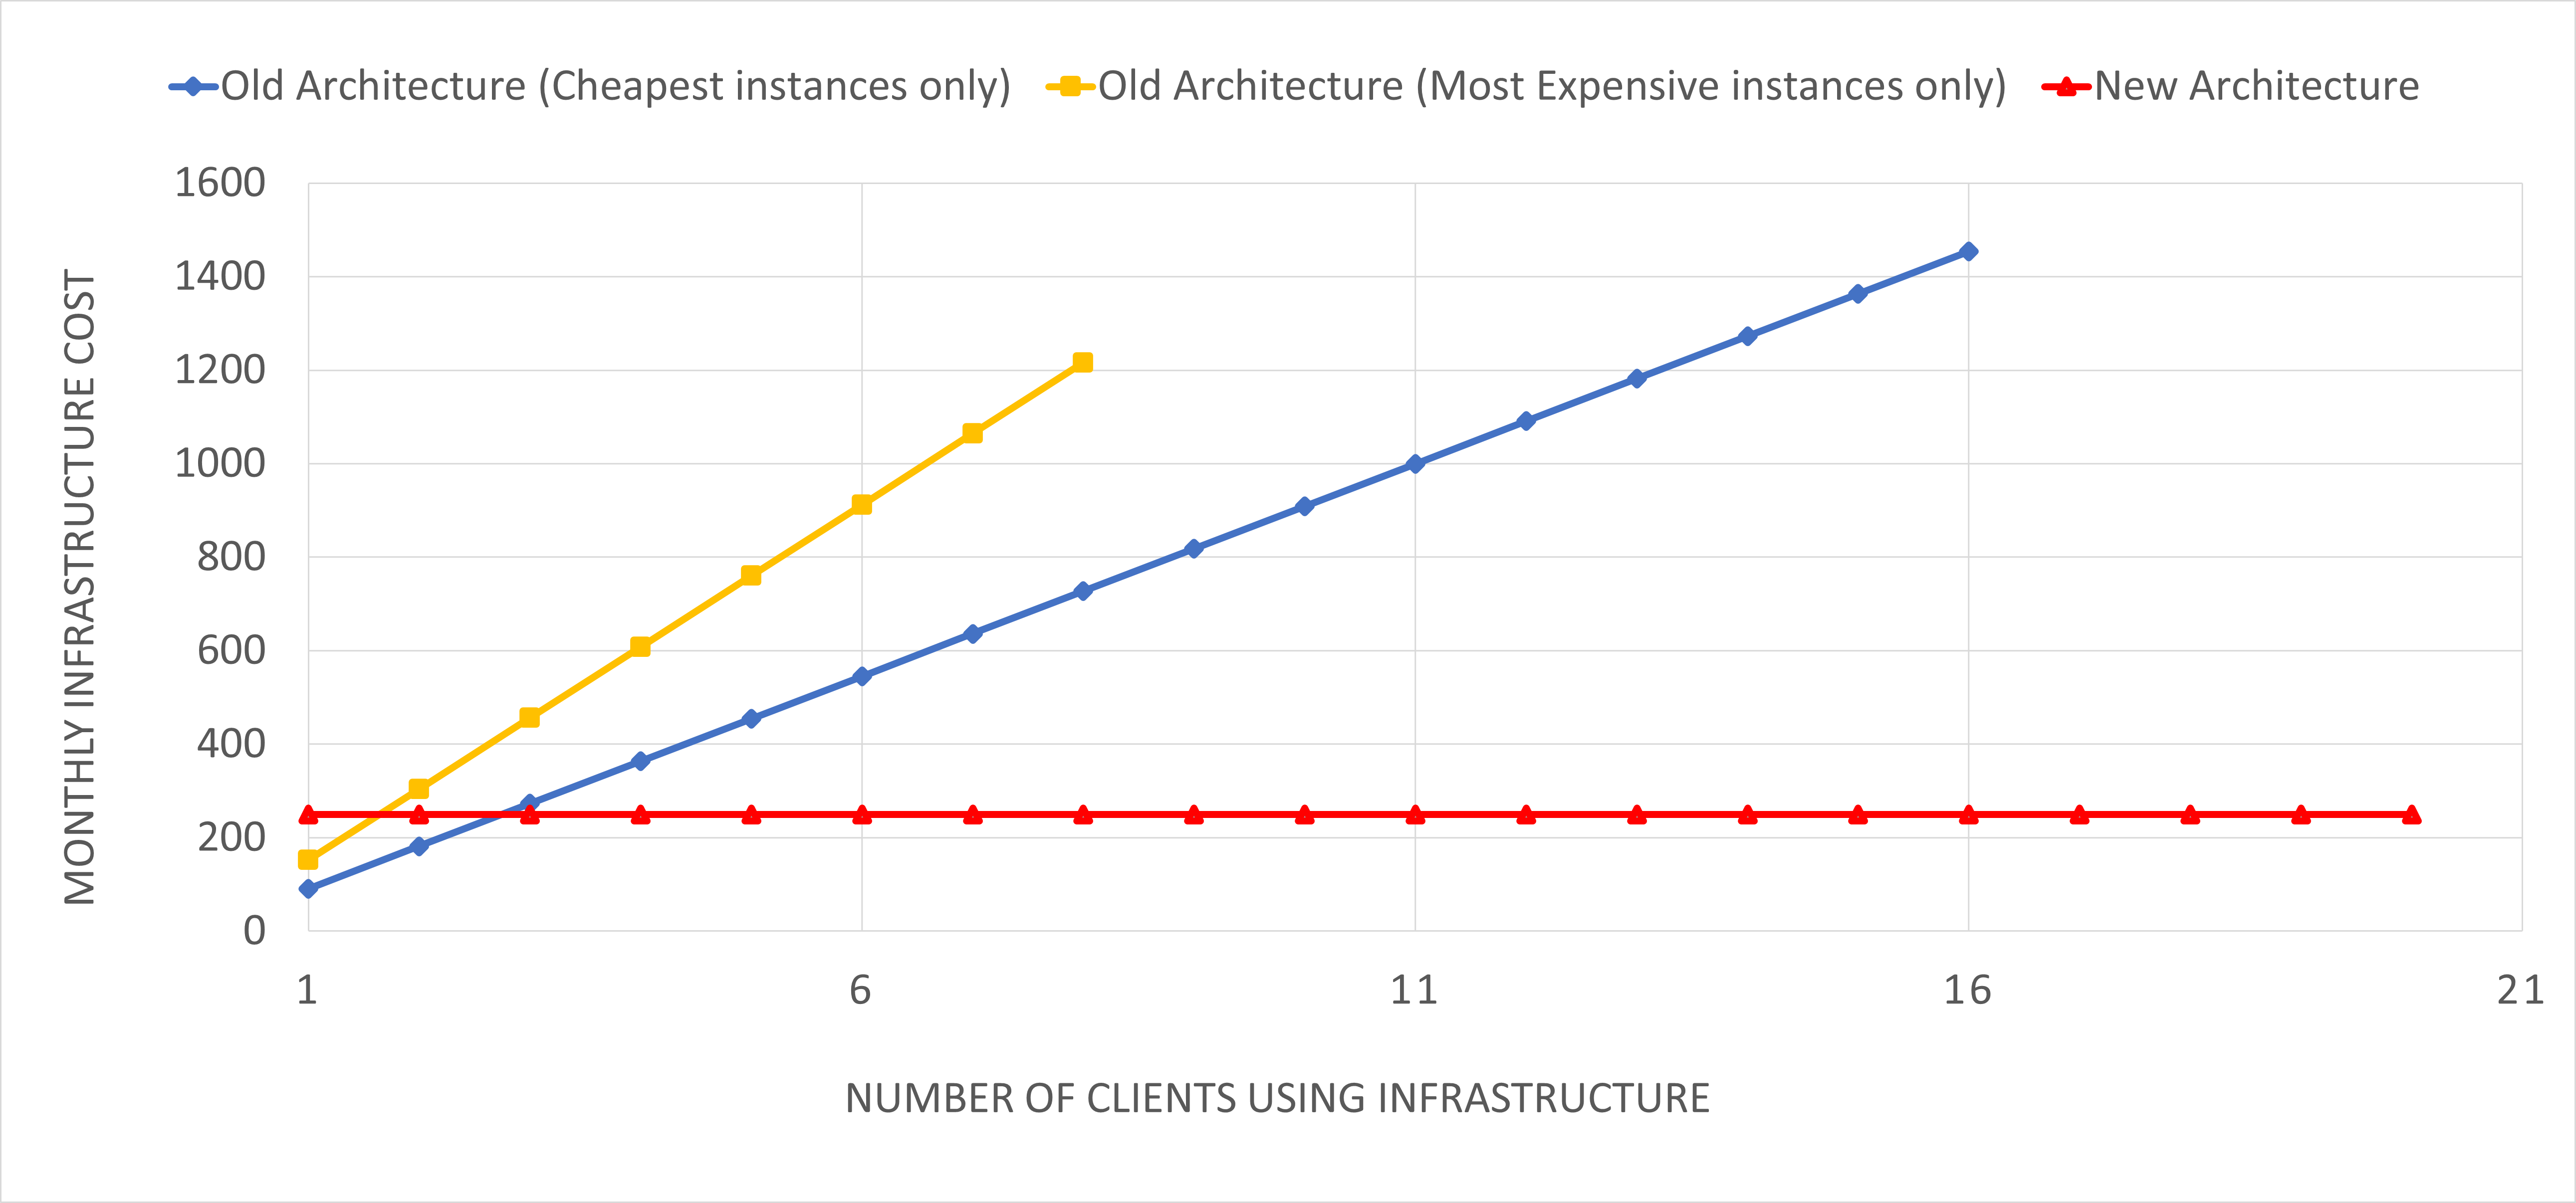
\includegraphics[width=0.95\textwidth]{img/charts/infra-cost-per-client.png}}
    \caption[Infrastructure Cost Per Client]{Infrastructure Cost Per Client.}
    \label{fig:infra-cost-per-client}
\end{figure} 
    

As mentioned in \cref{methodology:sss:scaling}, due to constraints in the AWS EC2 service, there is a maximum limit of 32 \gls{vcpu} units for each AWS account. This means that, even if all of the Clients only required the smaller option that uses 2 \gls{vcpu}, the maximum number of Clients would still be only 16 Clients. With the new architecture, there is no hard limit on the number of clients that can be served simultaneously. As of the time of writing, the new architecture is currently serving three different clients, being that one of these Clients has a water network that generates as much data as all previous Clients combined, for both the old architecture and the new one. It was also tested using 17 fictional Clients, totaling 20 Clients being served by the Application simultaneously, with no discernible issues for the Users nor resource usages above the normal everyday operation with the three regular Clients.

The new architecture has one Application for each development environment --- Production, Staging and Internal. Using \Cref{tab:individual-cost-aws-new} as reference, each Environment uses two containers of type A for the PostgreSQL database and Redis services, two containers of type B for Backend API and InfluxDB database services, one container of type C and D for the Forecasting and KPI Calculation services, respectively. Finally, type E containers are used for the Optimization service. In order to test reducing even further the resource usage for services that are running constantly, in the Internal environment, the Backend API service and InfluxDB database service have been scaled down vertically to use containers of type A. Additionally, other services are being run in this Internal environment for further testing, but are not accounted here due to being temporary services used while the Web Platform is not ready for Production.



As can be observed in \cref{fig:infra-cost-per-client}, the monthly cost of maintaining the infrastructure needed for the Application scales linearly for the old architecture, while the new architecture's cost for low amounts of Clients is kept steady. Despite the fact that the new infrastructure has not yet been tested for more than 20 Clients, hence the data in the figure ending at 20 clients, according to the resource usage during both peak hours and idle times, these were largely unaltered, and usage difference was negligible. Therefore, the usage of the Application using the new architecture is sure to be capable of handling many more Clients simultaneously.


\subsubsection{Remaining Costs}\label{results-and-discussion:sss:remaining-costs}

The costs presented here are only the main costs associated with the differences between the architectures. These are the bulk of the monthly costs with the infrastructure used.
There are also costs related to Data Transfer in and out of the \gls{vpc}, costs with Costumer Support, costs associated with automatic backups of data and other resources. Some resource usages are not reported in this document due to Client confidentiality agreements, being free of charge or being used so sparingly or in low quantities that the costs are irrelevant or included in the Free Tier\footnote{Certain AWS resources are free until a certain level of usage is achieved.}.

\subsection{Development and Deployment Issues}

Besides the infrastructural scaling issue, there was also a problem scaling the human resources needed for development. Having the Application be the same for all of the Clients, instead of being one separately maintained Application for each Client, drastically lowers the developer manpower needed for maintaining and updating an Application for multiple Clients. Therefore, this new architecture is substantially and clearly scalable when compared with the previous architecture.

\section{DevOps Improvements}\label{results-and-discussion:ss:devops-improvements}

The Company's developer team's general sentiment towards the implementation of the new architecture is one of relief and excitement. As stated in \Cref{methodology:sss:deployments} and \cref{methodology:sss:testing}, there were several issues regarding the developer workflow when working in the Application. After implementing the new architecture, these concerns have diminished considerably. The measures taken in \cref{methodology:ss:solving-the-deployment-issues} and \Cref{methodology:sss:testing-new} have brought a new and better workflow to the development team. This can be attested by the results in the \gls{fkm}.



\section{Observability Improvements}\label{results-and-discussion:ss:observability-improvements}

\textcolor{orange}{Here, show some dashboards of the observability system, exemplifying normal day-to-day operation, error detection, etc...}

